\section{Methodology: $RtSEngine$ Framework}
\label{sec:method}
%
%\blue{how this section is org, 2-3 sentences, later when this whole section is completed.}
%
The goal of $RtSEngine$ is to recommend a set of aggregate views that are considered interesting because of their abnormal deviations.
%
%Also, the recommendation process will be tuned with certain realtime limits, i.e., number of explored views $R$ and execution time $tl$.
% 
To achieve that, $RtSEngine$ utilizes the following key idea: recommend views that are created from grouping high ranked dimension attributes $A'$ within the set $A$.
%
The attributes ranks in $A'$ are computed using our proposed prioritizing techniques discussed later in the following sections.
%
%The suggested aggregate views are created from grouping high ranked dimension attributes which evaluated using our proposed prioritizing techniques presented in section \ref{sec:method}. 
Essentially, those techniques evaluate the priorities of all dimension attributes according to their statistical features gathered from the meta-data, e.g., number of selected values, data distribution, and selectivity.
% 
Then, by reordering all dimension attributes according to their priorities, only a subset of high priority attributes are passed to the execution engine, hence, limiting the number of examined views and execution time.  

Conceptually, $RtSEngine$ \footnote{Implementations and data are available at:\\ https://github.com/ibrahimDKE/Cdb\_RtsEngine\_DKE\_UQ},is designed as a recommendation plug-in that can be applied to any visualization engine, e.g., Tableau and Spotfire.
%
However, in this work, we built $RtSEngine$ as a standalone end-to-end system on top of SeeDB which allows users to pose arbitrary queries over data and obtain recommended visualizations.
%
%\mas{again, cost estimation is not a contribution, it is just a parameter. It is pretty much the same as estimating number of distinct values}
$RtSEngine$ is comprised of two main modules (See Figure \ref{fig:arch}):
%
\begin{figure}[t]
\centering
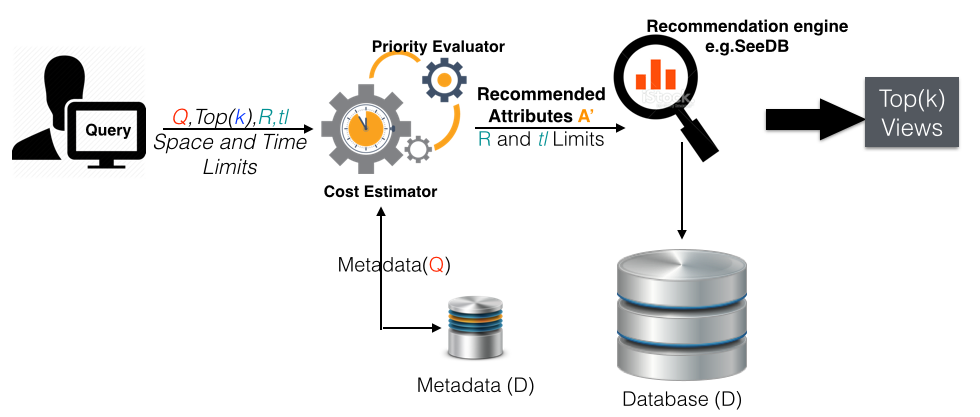
\includegraphics[width=\textwidth]{arch_new.png}
%\subfloat[fig2:Accuracy] {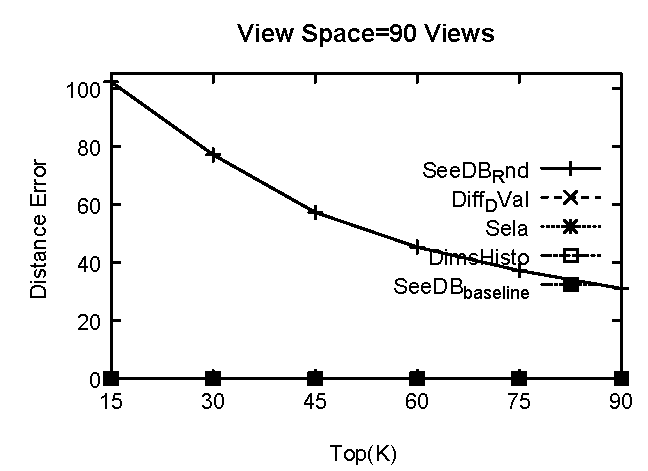
\includegraphics[width=2in]{12.pdf}}
\caption{$RtSEngine$: Real time Evaluation Architecture for Automatic recommendation}
\label{fig:arch}%
\end{figure}
%
\begin{enumerate}
\item \textbf{Priority Evaluator:} An underlying module in front of any recommendation engine. 
%
Used to evaluate the dimension attributes that form visualizations according to a priority function $Pr$ computed using our proposed techniques.
%
\item \textbf{Cost Estimator:} This module is supposed to run in parallel with the Priority Evaluator to estimate the retrieval and computation costs of each visualization using our estimation approaches. 
%
Estimating the visualization costs in real-time improves the efficiency by discounting high costs and low priorities visualizations. 
%
Note that this module is an awareness cost approach which incorporates the estimated costs to assess visualizations based on their priorities and costs.
%
\end{enumerate}
%
We define a notion of benefits $Benefit(V_i)$ of a view $V_i$ as the gains from each view represented as the utility of view $U(V_i)$, compared with the time spent $Cost(V_i)$ to compute the view $V_i$.
%
Formally:
%
\begin{equation}
\label{eq:profit}
Benefit(V_i)= \frac{U(V_i)}{Cost(V_i)}
\end{equation}
%

Cost estimations of visualizations is discussed later on Section \ref{sec:cost_est}.
%
Both modules (Priority Evaluator and Cost Estimator) read information by querying metadata to collect information about dimension attributes, e.g., number of distinct values and cardinality.
%
Next, we describe the two modules in details.
%
%\subsection{Priority Evaluator: Dimension Attributes Prioritizing}%
%\label{sec:priority_evaluator}
%
%\subsection{Cost Estimator: Visualizations Cost Estimation}
%\label{cost_estimator}
%